\documentclass[usenames,dvipsnames]{beamer}
\usepackage{../../shared/styles/custom}
% =============================================================================
% ML TEACHING MATHEMATICAL NOTATION CONVENTIONS
% =============================================================================
% Based on standard ML textbooks: Murphy's "Machine Learning: A Probabilistic Perspective",
% Bishop's "Pattern Recognition and Machine Learning", and "Mathematics for Machine Learning"

% =============================================================================
% CORE NOTATION STANDARDS
% =============================================================================

% SCALARS: Regular italics (lowercase for variables, uppercase for constants)
% Examples: x, y, n, d, k, \theta, \alpha, \lambda, \sigma

% VECTORS: Bold lowercase letters
% Examples: \mathbf{x}, \mathbf{w}, \mathbf{\mu}, \mathbf{\theta}

% MATRICES: Bold uppercase letters
% Examples: \mathbf{X}, \mathbf{W}, \mathbf{\Sigma}, \mathbf{\Lambda}

% SETS: Calligraphic uppercase
% Examples: \mathcal{D}, \mathcal{X}, \mathcal{Y}

% SPACES: Blackboard bold
% Examples: \mathbb{R}, \mathbb{Z}, \mathbb{N}

% =============================================================================
% VECTOR NOTATION (bold lowercase)
% =============================================================================

\newcommand{\vx}{\mathbf{x}}        % Input vector
\newcommand{\vy}{\mathbf{y}}        % Output vector
\newcommand{\vw}{\mathbf{w}}        % Weight vector
\newcommand{\vb}{\mathbf{b}}        % Bias vector
\newcommand{\vh}{\mathbf{h}}        % Hidden vector
\newcommand{\vz}{\mathbf{z}}        % Latent vector
\newcommand{\vf}{\mathbf{f}}        % Function vector
\newcommand{\vg}{\mathbf{g}}        % Gradient vector
\newcommand{\vu}{\mathbf{u}}        % Generic vector u
\newcommand{\vv}{\mathbf{v}}        % Generic vector v
\newcommand{\vzero}{\mathbf{0}}     % Zero vector
\newcommand{\vone}{\mathbf{1}}      % Ones vector

% Greek vectors (bold)
\newcommand{\vmu}{\boldsymbol{\mu}}     % Mean vector
\newcommand{\vtheta}{\boldsymbol{\theta}} % Parameter vector
\newcommand{\vlambda}{\boldsymbol{\lambda}} % Lambda vector
\newcommand{\valpha}{\boldsymbol{\alpha}}   % Alpha vector
\newcommand{\vbeta}{\boldsymbol{\beta}}     % Beta vector
\newcommand{\vxi}{\boldsymbol{\xi}}         % Xi vector
\newcommand{\vepsilon}{\boldsymbol{\epsilon}} % Epsilon vector

% =============================================================================
% MATRIX NOTATION (bold uppercase)
% =============================================================================

\newcommand{\mX}{\mathbf{X}}        % Data matrix
\newcommand{\mY}{\mathbf{Y}}        % Target matrix
\newcommand{\mW}{\mathbf{W}}        % Weight matrix
\newcommand{\mA}{\mathbf{A}}        % Generic matrix A
\newcommand{\mB}{\mathbf{B}}        % Generic matrix B
\newcommand{\mC}{\mathbf{C}}        % Generic matrix C
\newcommand{\mH}{\mathbf{H}}        % Hidden layer matrix / Hessian
\newcommand{\mI}{\mathbf{I}}        % Identity matrix
\newcommand{\mJ}{\mathbf{J}}        % Jacobian matrix
\newcommand{\mK}{\mathbf{K}}        % Kernel matrix
\newcommand{\mL}{\mathbf{L}}        % Loss matrix / Cholesky factor
\newcommand{\mP}{\mathbf{P}}        % Projection matrix
\newcommand{\mQ}{\mathbf{Q}}        % Orthogonal matrix
\newcommand{\mR}{\mathbf{R}}        % Rotation matrix
\newcommand{\mS}{\mathbf{S}}        % Scatter matrix
\newcommand{\mU}{\mathbf{U}}        % Left singular vectors
\newcommand{\mV}{\mathbf{V}}        % Right singular vectors

% Greek matrices (bold)
\newcommand{\mSigma}{\boldsymbol{\Sigma}}   % Covariance matrix
\newcommand{\mLambda}{\boldsymbol{\Lambda}} % Diagonal eigenvalue matrix
\newcommand{\mPhi}{\boldsymbol{\Phi}}       % Feature matrix
\newcommand{\mPsi}{\boldsymbol{\Psi}}       % Basis matrix
\newcommand{\mTheta}{\boldsymbol{\Theta}}   % Parameter matrix

% =============================================================================
% SETS AND SPACES (following Bishop/Murphy conventions)
% =============================================================================

\newcommand{\cD}{\mathcal{D}}       % Dataset
\newcommand{\cH}{\mathcal{H}}       % Hypothesis space
\newcommand{\cX}{\mathcal{X}}       % Input space
\newcommand{\cY}{\mathcal{Y}}       % Output space
\newcommand{\cF}{\mathcal{F}}       % Function space
\newcommand{\cG}{\mathcal{G}}       % Gaussian process
\newcommand{\cL}{\mathcal{L}}       % Lagrangian / Loss
\newcommand{\cN}{\mathcal{N}}       % Normal distribution
\newcommand{\cU}{\mathcal{U}}       % Uniform distribution
\newcommand{\cB}{\mathcal{B}}       % Bernoulli distribution
\newcommand{\cP}{\mathcal{P}}       % Probability distribution

% Number systems
\newcommand{\Real}{\mathbb{R}}      % Real numbers
\newcommand{\Nat}{\mathbb{N}}       % Natural numbers
\newcommand{\Int}{\mathbb{Z}}       % Integers
\newcommand{\Complex}{\mathbb{C}}   % Complex numbers

% =============================================================================
% OPERATORS AND FUNCTIONS (following standard conventions)
% =============================================================================

% Prediction notation (commonly used in ML)
\newcommand{\yhat}{\hat{\vy}}        % Predicted output vector (bold)
\newcommand{\yhati}{\hat{y}_i}       % Predicted output for sample i (scalar)

% Common ML functions (with conflict resolution)
\providecommand{\sigmoid}{}
\renewcommand{\sigmoid}{\operatorname{sigmoid}}
\providecommand{\softmax}{}
\renewcommand{\softmax}{\operatorname{softmax}}
\providecommand{\ReLU}{}
\renewcommand{\ReLU}{\operatorname{ReLU}}
\providecommand{\sign}{}
\renewcommand{\sign}{\operatorname{sign}}
\DeclareMathOperator{\Gain}{Gain}    % Information gain
\DeclareMathOperator{\Entropy}{Entropy}
% KL divergence (check for conflicts)
\providecommand{\KL}{}
\renewcommand{\KL}{\operatorname{KL}}
\DeclareMathOperator{\MSE}{MSE}      % Mean squared error
\DeclareMathOperator{\MAE}{MAE}      % Mean absolute error
\DeclareMathOperator{\RMSE}{RMSE}    % Root mean squared error

% Classification metrics (upright text)
\newcommand{\TP}{\text{TP}}          % True positives
\newcommand{\TN}{\text{TN}}          % True negatives  
\newcommand{\FP}{\text{FP}}          % False positives
\newcommand{\FN}{\text{FN}}          % False negatives
\DeclareMathOperator{\Precision}{Precision}
\DeclareMathOperator{\Recall}{Recall}
\DeclareMathOperator{\Accuracy}{Accuracy}

% Transpose and inverse
\newcommand{\tp}{^\top}             % Transpose (Bishop/Murphy style)
\newcommand{\inv}{^{-1}}            % Matrix inverse
\newcommand{\pinv}{^{\dagger}}      % Pseudoinverse

% Norms (consistent with Murphy/Bishop)
\newcommand{\norm}[1]{\|#1\|}       % Generic norm
\newcommand{\normone}[1]{\|#1\|_1}  % L1 norm
\newcommand{\normtwo}[1]{\|#1\|_2}  % L2 norm
\newcommand{\norminf}[1]{\|#1\|_\infty} % L-infinity norm
\newcommand{\normF}[1]{\|#1\|_F}    % Frobenius norm

% Optimization operators (upright as in Murphy)
\providecommand{\argmin}{}
\renewcommand{\argmin}{\operatorname*{arg\,min}}
\providecommand{\argmax}{}
\renewcommand{\argmax}{\operatorname*{arg\,max}}
\DeclareMathOperator{\minimize}{minimize}
\DeclareMathOperator{\maximize}{maximize}
\DeclareMathOperator{\subjectto}{subject\,to}

% Matrix operations (upright) - use conditional definitions
\providecommand{\tr}{}
\renewcommand{\tr}{\operatorname{tr}}       % Trace
\providecommand{\det}{}
\renewcommand{\det}{\operatorname{det}}     % Determinant
\providecommand{\rank}{}
\renewcommand{\rank}{\operatorname{rank}}   % Rank
\providecommand{\span}{}
\renewcommand{\span}{\operatorname{span}}   % Span
\providecommand{\null}{}
\renewcommand{\null}{\operatorname{null}}   % Null space
\DeclareMathOperator{\range}{range} % Range/column space
\providecommand{\diag}{}
\renewcommand{\diag}{\operatorname{diag}}   % Diagonal operator
\providecommand{\vec}{}
\renewcommand{\vec}{\operatorname{vec}}     % Vectorization operator

% Probability and statistics (Murphy/Bishop style)
\newcommand{\Prob}{\mathbb{P}}      % Probability measure
\newcommand{\Exp}{\mathbb{E}}       % Expectation
\DeclareMathOperator{\Var}{Var}     % Variance
\DeclareMathOperator{\Cov}{Cov}     % Covariance
\DeclareMathOperator{\Corr}{Corr}   % Correlation
% KL divergence already defined above
\DeclareMathOperator{\MI}{I}        % Mutual information

% Activation functions (already defined above with conflict resolution)

% =============================================================================
% STANDARD PARAMETER CONVENTIONS (Murphy/Bishop style)
% =============================================================================

% Primary parameters: θ (theta) - following Murphy's convention
% Learning rates: α, η (alpha, eta)
% Regularization: λ (lambda)
% Precision: β (beta) - following Bishop
% Variance: σ² (sigma squared)
% Standard deviation: σ (sigma)
% Mean: μ (mu)

% Common scalars:
% n - number of training examples
% d - dimensionality of input
% k - number of classes/clusters
% m - number of hidden units
% T - number of time steps
% i, j - indices

% =============================================================================
% STANDARD NOTATION EXAMPLES (Murphy/Bishop style)
% =============================================================================

% Linear regression:      y = \vw\tp\vx + b
% Matrix form:            \vy = \mX\vw + b\vone
% Logistic regression:    p(y=1|\vx) = \sigmoid(\vw\tp\vx)
% Gaussian:               \vx \sim \cN(\vmu, \mSigma)
% Parameter update:       \vtheta_{t+1} = \vtheta_t - \alpha \nabla \cL(\vtheta_t)
% Likelihood:             p(\cD|\vtheta) = \prod_{i=1}^n p(y_i|\vx_i, \vtheta)
% Posterior:              p(\vtheta|\cD) \propto p(\cD|\vtheta)p(\vtheta)
% Prediction:             p(y^*|\vx^*, \cD) = \int p(y^*|\vx^*, \vtheta)p(\vtheta|\cD)d\vtheta

% =============================================================================
% COMMON MISTAKES TO AVOID
% =============================================================================

% ❌ WRONG NOTATION          →  ✅ CORRECT NOTATION (Murphy/Bishop style)

% Transpose:
% ❌ x^t, X^t              →  ✅ \vx\tp, \mX\tp
% ❌ x', X'                →  ✅ \vx\tp, \mX\tp

% Vectors vs Matrices vs Scalars:
% ❌ X (for vector)        →  ✅ \vx (bold lowercase)
% ❌ w (for weight vector) →  ✅ \vw (bold lowercase)
% ❌ x (for data matrix)   →  ✅ \mX (bold uppercase)
% ❌ \mathbf{\theta}       →  ✅ \vtheta (Greek vectors are bold)
% ❌ \mathbf{n}            →  ✅ n (scalars are not bold)

% Sets and distributions:
% ❌ R                     →  ✅ \Real (blackboard bold for number systems)
% ❌ \mathcal{R}           →  ✅ \Real (use blackboard for reals)
% ❌ Normal               →  ✅ \cN (calligraphic for distributions)

% Functions and operators:
% ❌ argmax                →  ✅ \argmax (upright operator)
% ❌ E[X]                  →  ✅ \Exp[X] (blackboard E for expectation)
% ❌ trace(A)              →  ✅ \tr(\mA) (upright operator)

% =============================================================================
% ALGORITHM NAME CONVENTIONS
% =============================================================================

% Use standard capitalizations as in textbooks:
% k-NN, SVM, PCA, GMM, EM, MAP, ML, SGD, Adam, RMSprop
% ReLU, tanh, sigmoid, softmax

\endinput

\usepackage{color, colortbl}
\usepackage{comment}

\newcommand*{\mathcolor}{}
\def\mathcolor#1#{\mathcoloraux{#1}}
\newcommand*{\mathcoloraux}[3]{%
	\protect\leavevmode
	\begingroup
	\color#1{#2}#3%
	\endgroup
}




\def\checkmark{\tikz\fill[scale=0.4](0,.35) -- (.25,0) -- (1,.7) -- (.25,.15) -- cycle;} 



\newcommand{\DoTikzmark}[1]{%
	\tikz[remember picture] \coordinate[shift={(0,.7ex)}](#1);%
}

\newcommand{\colrow}[3][]{%
	\tikz[overlay,remember picture, line width=10pt]
	\draw[shorten >=-.1em, shorten <=-.1em, #1] (#2)--(#3);
}


\newcolumntype{g}{>{\columncolor{Lavender}}c}
\newcolumntype{t}{>{\columncolor{Tan}}c}

%\beamerdefaultoverlayspecification{<+->}


	\ifx\relax#1\relax  \item \else \item[#1] \fi
	\abovedisplayskip=0pt\abovedisplayshortskip=0pt~\vspace*{-\baselineskip}}
	




\title{K-Nearest Neighbors}
\date{\today}
\author{Nipun Batra}
\institute{IIT Gandhinagar}
\begin{document}
  \maketitle

{
	\setbeamercolor{background canvas}{bg=}
	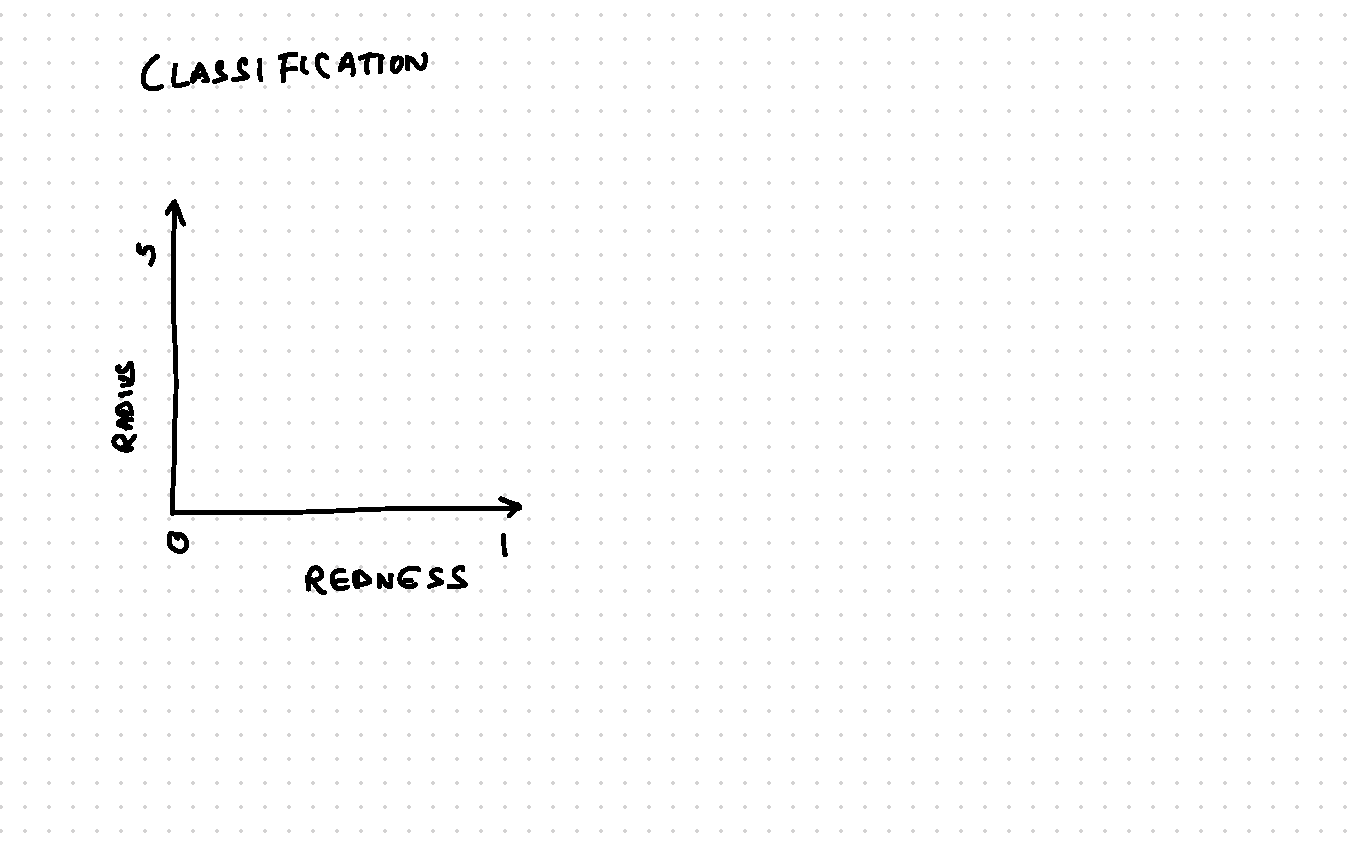
\includepdf[page=-]{../assets/knn/figures/knn-intuition.pdf}
}

{
	\setbeamercolor{background canvas}{bg=}
	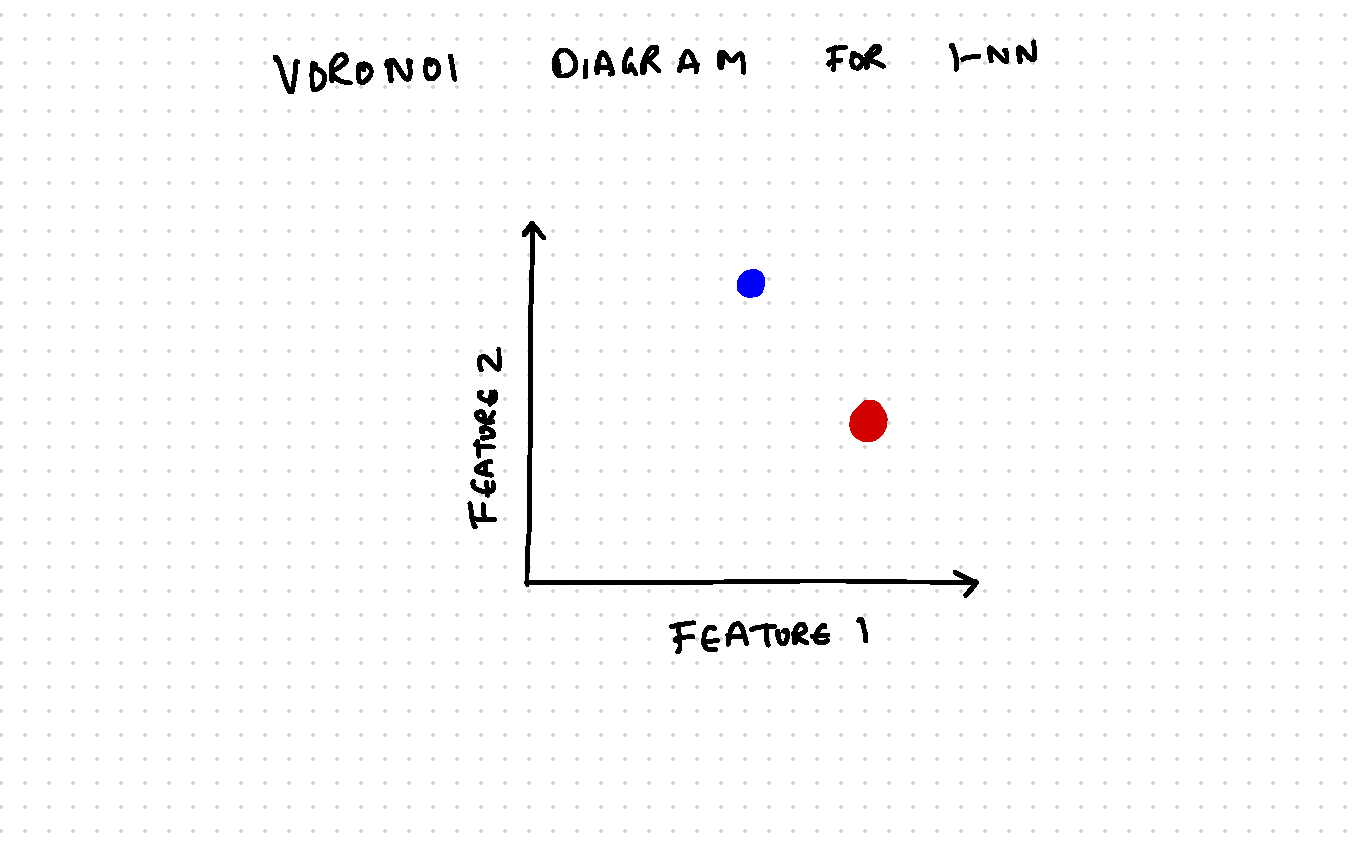
\includepdf[pages=1-25]{../assets/knn/figures/1nn.pdf}
}


\begin{frame}{Parametric vs Non-Parametric Models}
\begin{table}[]
\begin{tabular}{|l|p{3.5cm}|p{3.5cm}|}
\hline
            & Parametric                                               & Non-Parametric                                                   \\ \hline
Parameter   & Number of parameters is fixed w.r.t dataset size         & Number of parameters grows w.r.t. to an increase in dataset size \\ \hline
Speed       & Quicker (as the number of parameters are less)           & Longer (as number of parameters are less)                        \\ \hline
Assumptions & Strong Assumptions (like linearity in Linear Regression) & Very few (sometimes no) assumptions                              \\ \hline
Examples    & Linear Regression                                        & KNN, Decision Tree                     \\ \hline                         
\end{tabular}
\end{table}
\end{frame}

\begin{frame}{Lazy vs Eager Strategies}
	\begin{table}[]
		\begin{tabular}{|l|p{3.5cm}|p{3.5cm}|}
			\hline
			& Lazy                                     & Eager                                   \\
			\hline
			Train Time & $0$                                      & $\neq 0$                                \\
			\hline
			Test       & Long (due to comparison with train data) & Quick (as only ``parameters'' are involved) \\
			\hline
			Memory     & Store/Memorise entire data               & Store only learnt parameters            \\
			\hline
			Utility    & Useful for online settings               &                                         \\
			\hline
			Examples   & KNN                                      & Linear Regression, Decision Tree       \\ \hline
		\end{tabular}
	\end{table}
\end{frame}

\begin{frame}{Important Considerations}
\begin{itemize}
\item<1-> What are the \textbf{features} that will be considered for data similarity?
\item<2-> What is the \textbf{distance metric} that will be used to calculate data similarity?
\item<3-> What is the \textbf{aggregation function} that is going to be used?
\item<4-> What are the \textbf{number of neighbors} that you are going to take into consideration?
\item<5-> What is the \textbf{computational complexity} of the algorithm that you are implementing?
\end{itemize}
\end{frame}

\begin{frame}{Important Considerations: Distance Metric}
The Distance Metric acts as a \emph{measure of similarity} between the points.

{\centering
\only<2>{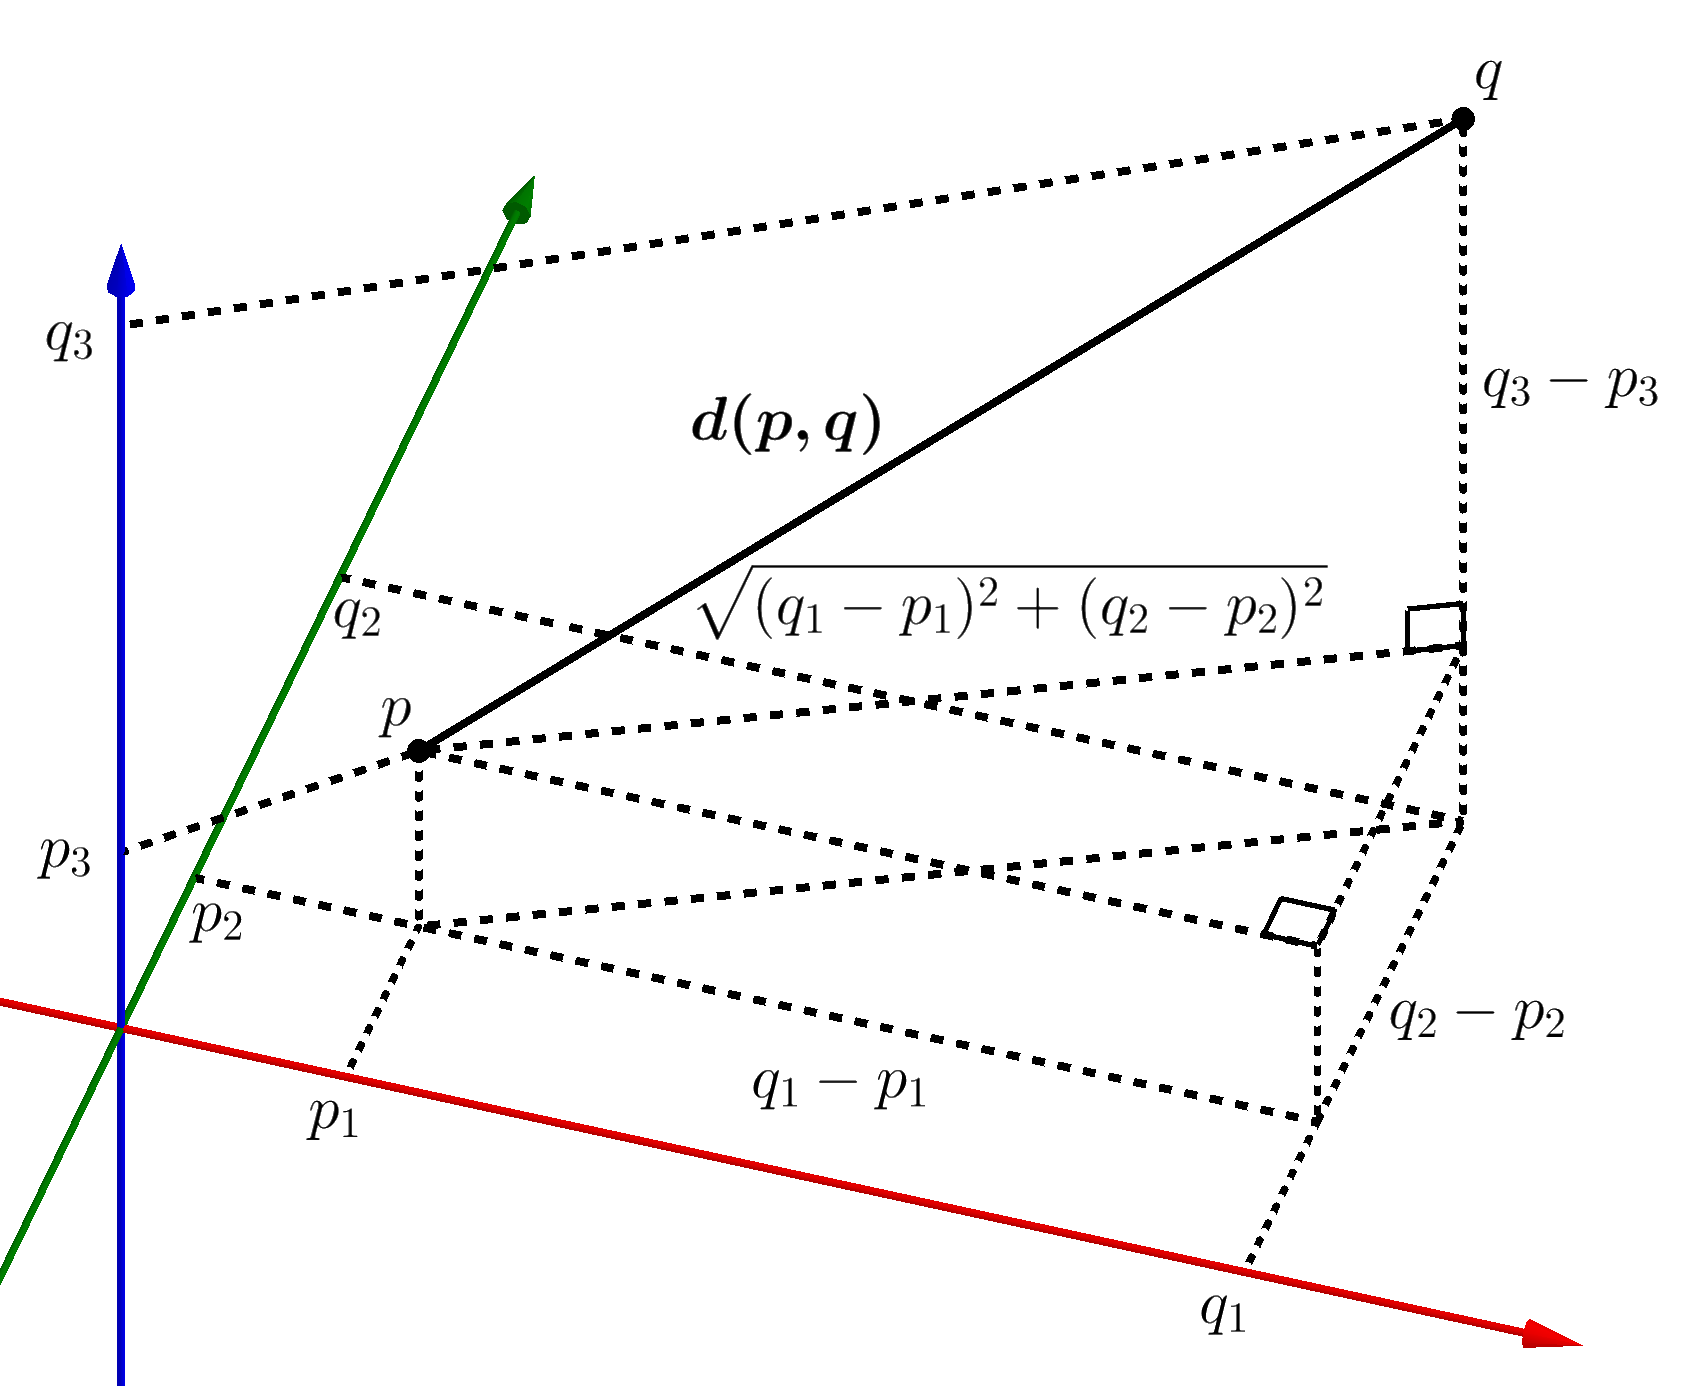
\includegraphics[height=0.6\textheight]{../assets/knn/figures/knn_ed.png}
\captionof{figure}{Euclidean Distance}}
\only<3>{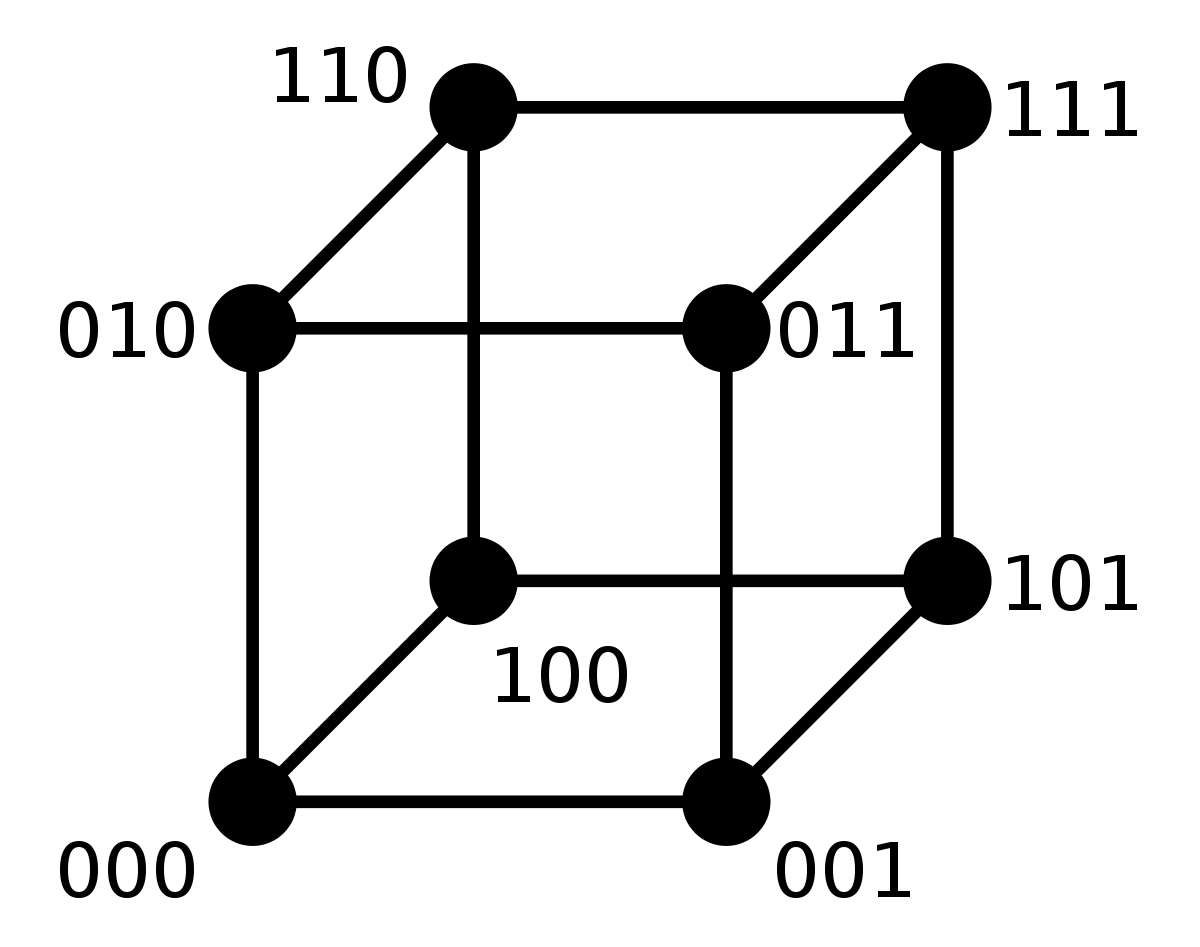
\includegraphics[height=0.6\textheight]{../assets/knn/figures/knn_hd.png}
\captionof{figure}{Hamming Distance}}
\only<4>{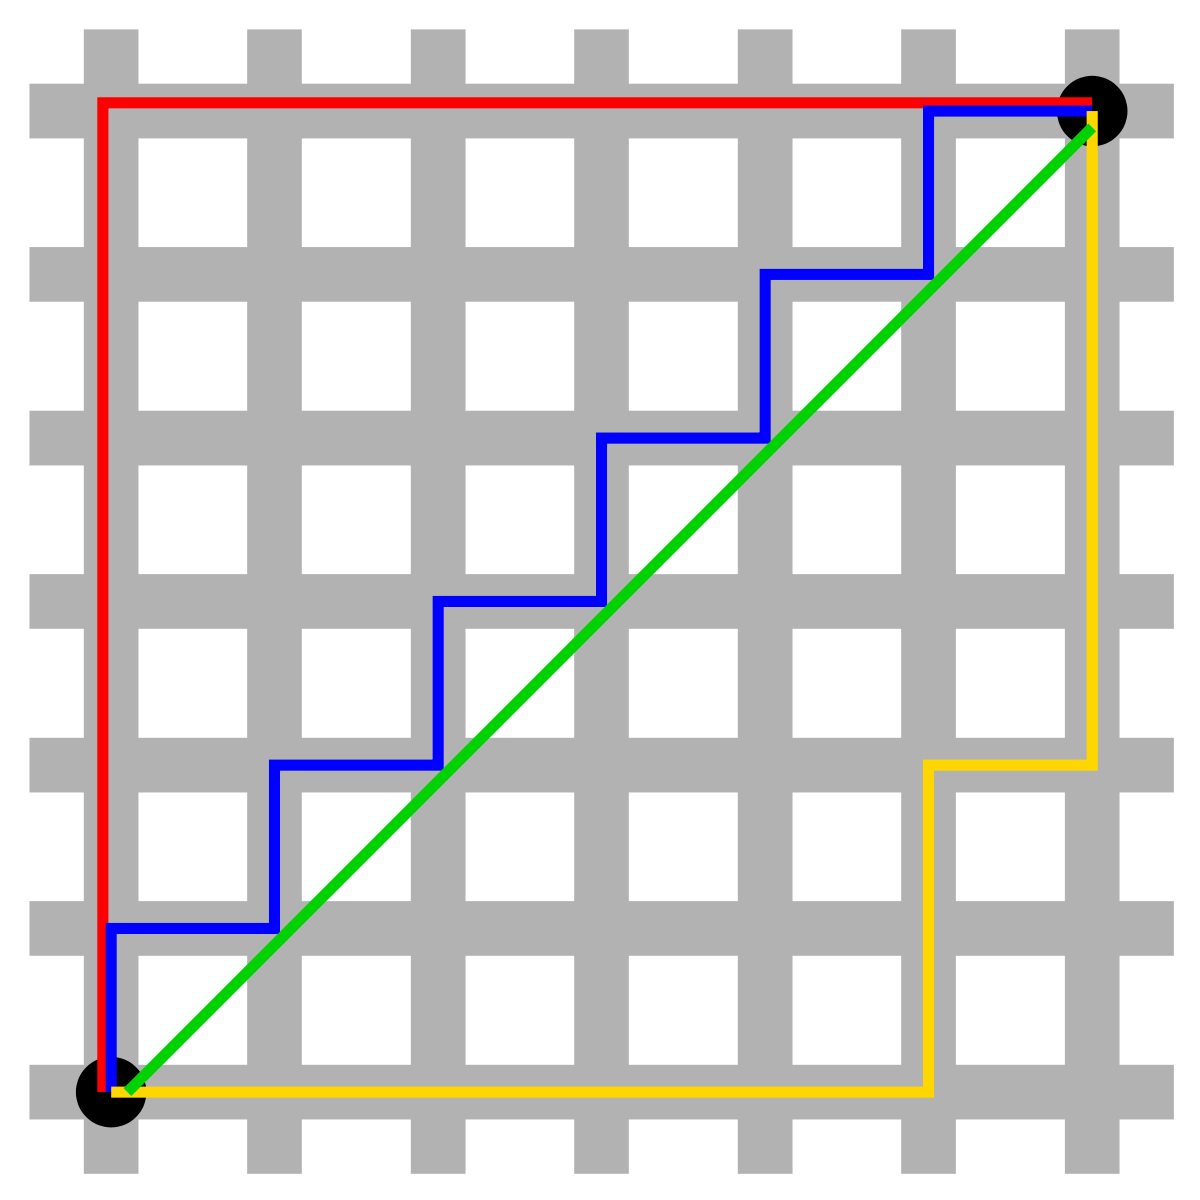
\includegraphics[height=0.6\textheight]{../assets/knn/figures/knn_md.png}
\captionof{figure}{Manhattan Distance}}}

%\only<5>{
%Choose the best distance metric \textbf{based on the properties of the data}. 

%Euclidean is a good distance measure to use if the input variables are similar in type (e.g. all measured widths and heights). Manhattan distance is a good measure to use if the input variables are not similar in type (such as age, gender, height, etc.).

%\href{https://machinelearningmastery.com/k-nearest-neighbors-for-machine-learning/}{More Info}}
\end{frame}


\begin{comment}


\begin{frame}{Important Considerations: Distance Metric}
Variation of decision boundaries of a random data set
\begin{figure}
    \centering
    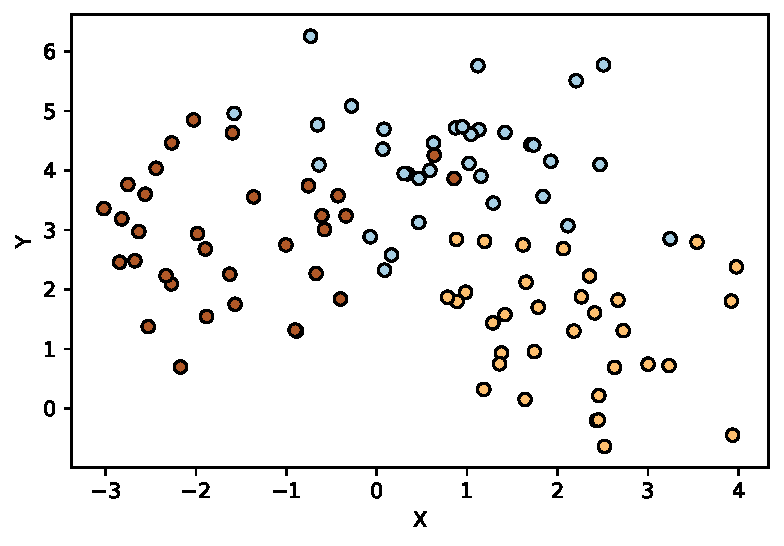
\includegraphics[width=0.6\linewidth]{../assets/knn/figures/iris_knn_data.pdf}
    \caption{Randomly generated blobs}
\end{figure}
\end{frame}

\begin{frame}{Important Considerations: Distance Metric}
\only<1>{
\begin{columns}[T]
  \begin{column}{0.5\textwidth}
    \begin{figure}
      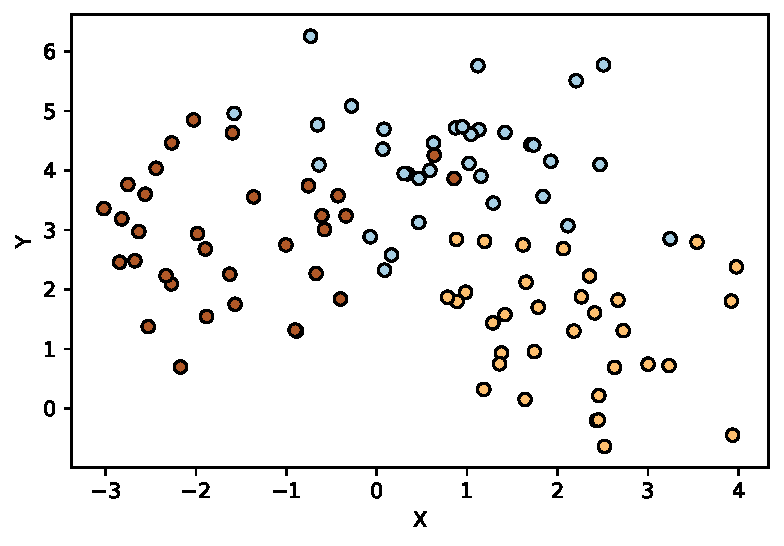
\includegraphics[width=\textwidth]{../assets/knn/figures/iris_knn_data.pdf}
      %\vspace*{-0.3cm}
      \caption{Ground Truth}
    \end{figure}
  \end{column}
  \begin{column}{0.5\textwidth}
    \begin{figure}
      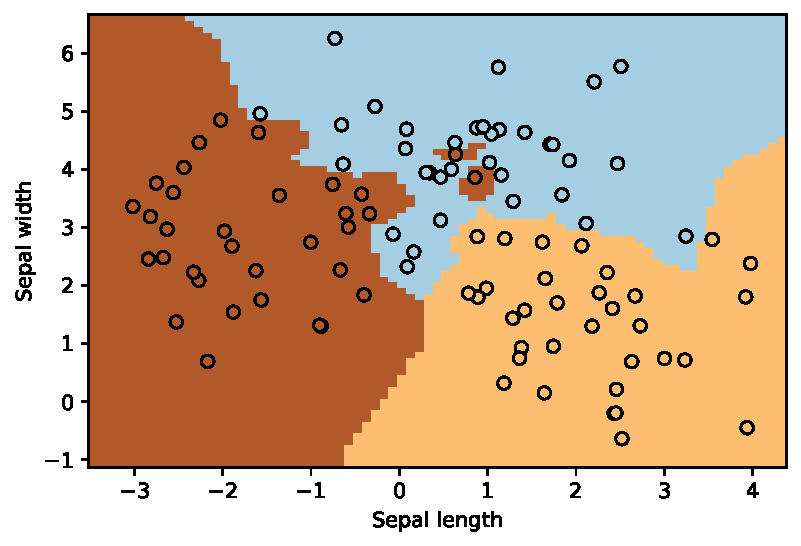
\includegraphics[width=\textwidth]{../assets/knn/figures/iris_knn_def_1.pdf}
      %\vspace*{-0.3cm}
      \caption{Minskoaski = $\left(\sum|x-y|^p\right)^{\frac{1}{p}}$}
    \end{figure}
  \end{column}
\end{columns}}
\only<2>{
\begin{columns}[T]
  \begin{column}{0.5\textwidth}
    \begin{figure}
      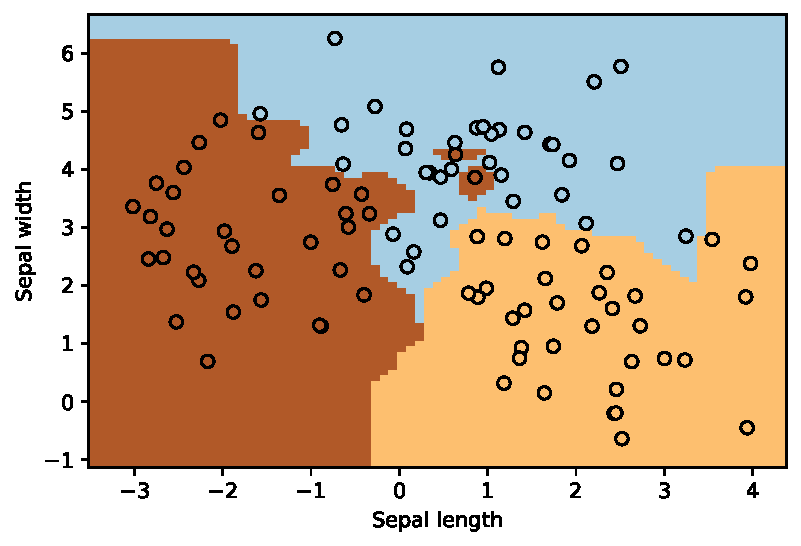
\includegraphics[width=\textwidth]{../assets/knn/figures/iris_knn_man_1.pdf}
      %\vspace*{-0.3cm}
      \caption{Manhattan = $\sum|x-y|$}
    \end{figure}
  \end{column}
  \begin{column}{0.5\textwidth}
    \begin{figure}
      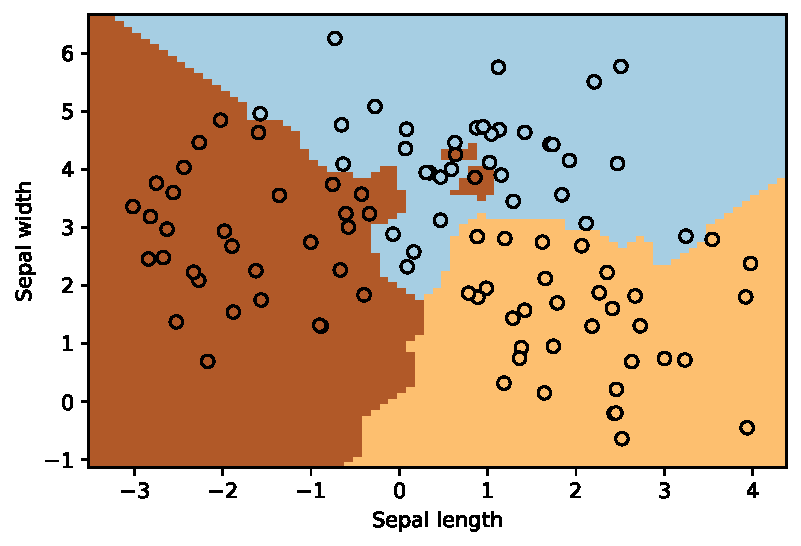
\includegraphics[width=\textwidth]{../assets/knn/figures/iris_knn_che_1.pdf}
      %\vspace*{-0.3cm}
      \caption{Chebeshev = $\max|x-y|$}
    \end{figure}
  \end{column}
\end{columns}}
\end{frame}
\end{comment}
\begin{frame}{Important Considerations: Value of \emph{K}}
Choosing the correct value of \emph{K} is difficult.
\pause

\textbf{Low values of K} will result in each point having a very high influence on the final output $\implies$ noise will influence the result
\pause

\textbf{High values of K} will result in smoother decision boundaries \\$\implies$ lower variance but also higher bias
\end{frame}

\begin{frame}{Important Considerations: Value of \emph{K}}
\only<1>{\begin{columns}[T]
  \begin{column}{0.5\textwidth}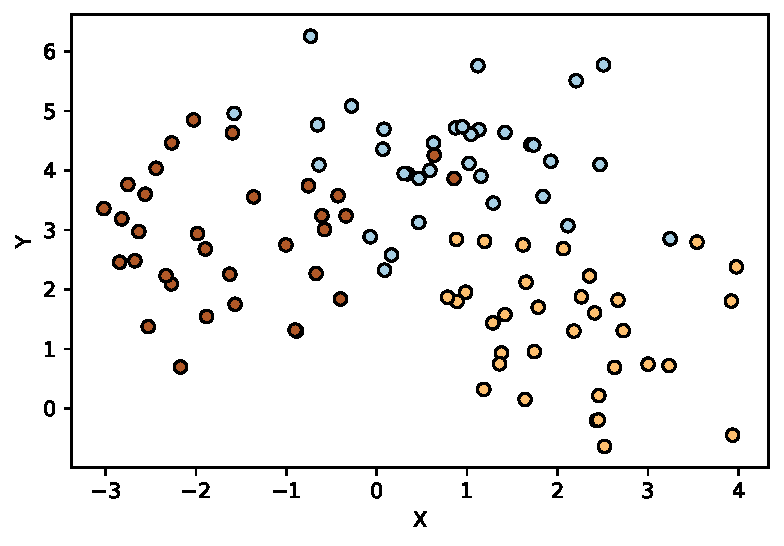
\includegraphics[height=0.7\textwidth]{../assets/knn/figures/iris_knn_data.pdf}\captionof{figure}{Dataset}\end{column}
  \begin{column}{0.5\textwidth}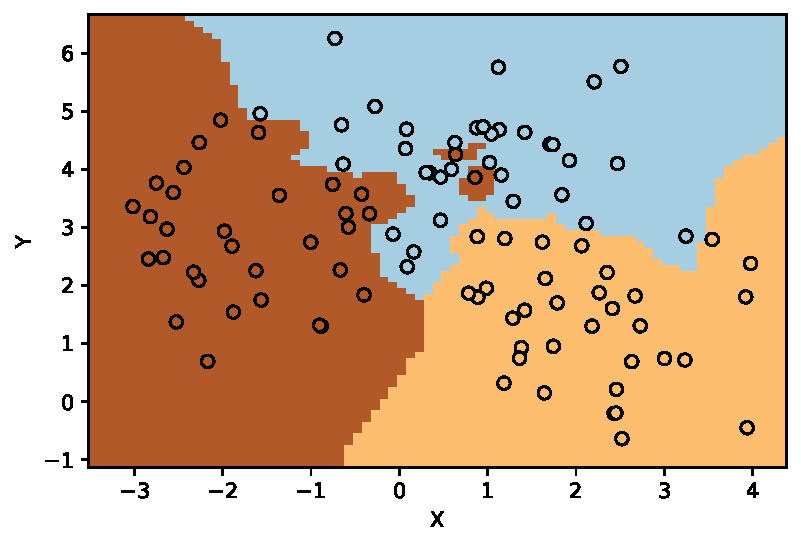
\includegraphics[height=0.7\textwidth]{../assets/knn/figures/exp_knn_1.pdf}\captionof{figure}{K = 1 High Variance}\end{column}\end{columns}}
\only<2>{\begin{columns}[T]
  \begin{column}{0.5\textwidth}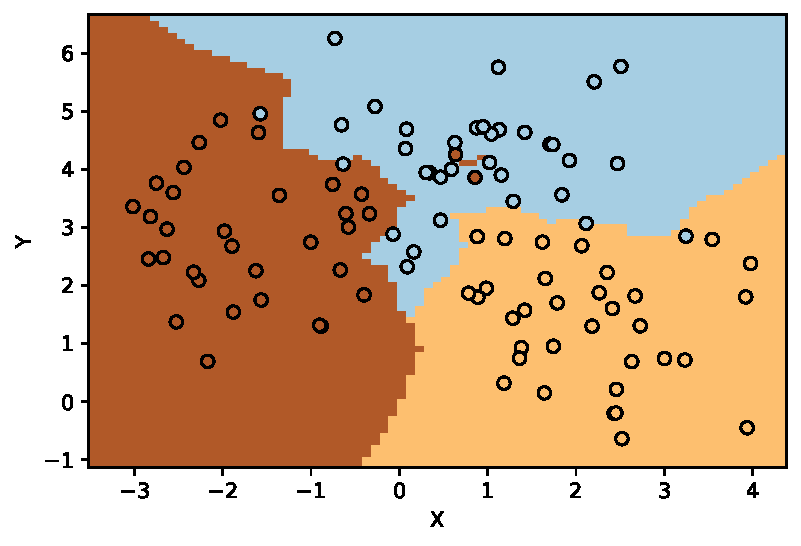
\includegraphics[height=0.7\textwidth]{../assets/knn/figures/exp_knn_3.pdf}\captionof{figure}{K = 3}\end{column}
  \begin{column}{0.5\textwidth}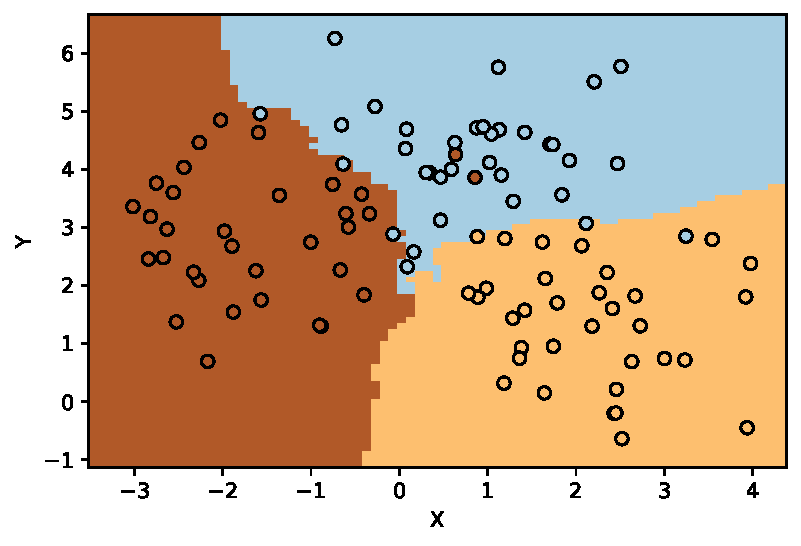
\includegraphics[height=0.7\textwidth]{../assets/knn/figures/exp_knn_9.pdf}\captionof{figure}{K = 9 High Bias}\end{column}\end{columns}}

\end{frame}

%\begin{frame}{Important Considerations: Value of \emph{K}}
%\only<1>{\begin{columns}[T]
%  \begin{column}{0.5\textwidth}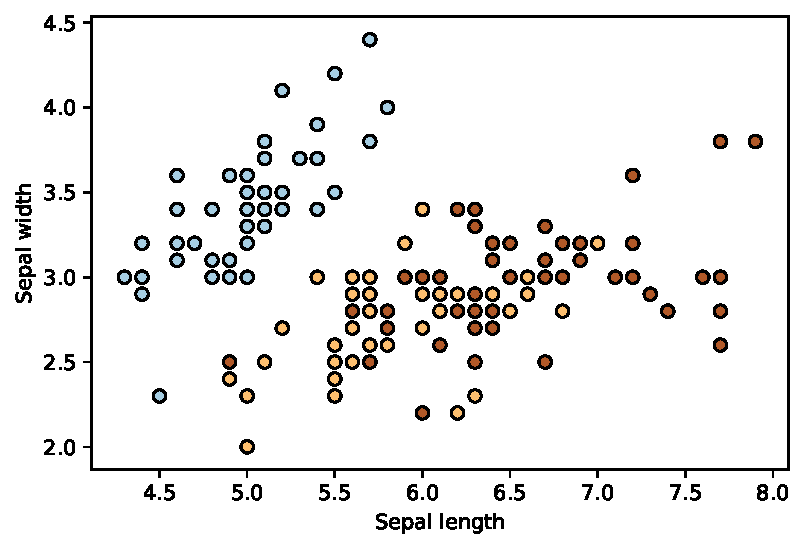
\includegraphics[height=0.7\textwidth]{../assets/knn/figures/iris.pdf}\captionof{figure}{Iris Dataset}\end{column}
%  \begin{column}{0.5\textwidth}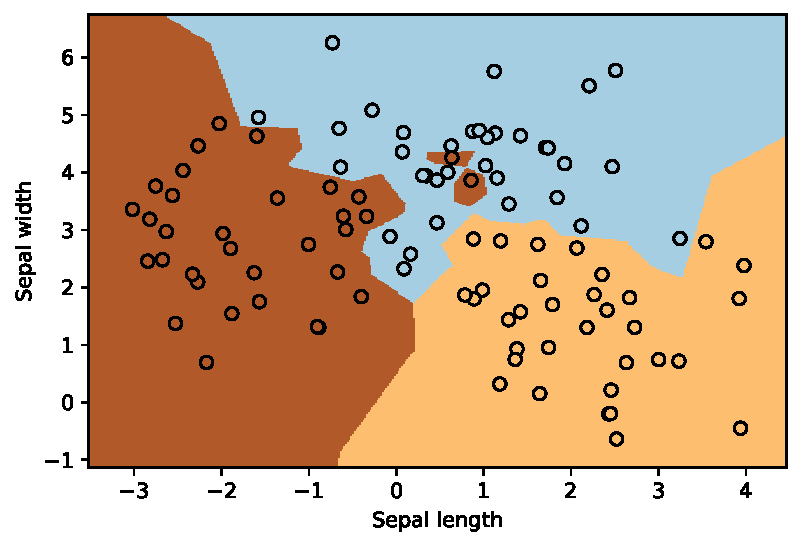
\includegraphics[height=0.7\textwidth]{../assets/knn/figures/iris_knn_1.pdf}\captionof{figure}{K = 1}\end{column}\end{columns}}
%\only<2>{\begin{columns}[T]
%  \begin{column}{0.5\textwidth}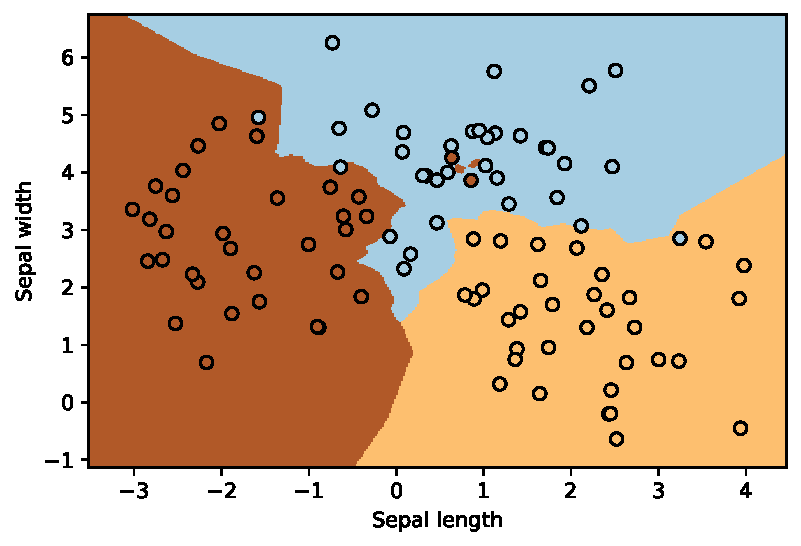
\includegraphics[height=0.7\textwidth]{../assets/knn/figures/iris_knn_3.pdf}\captionof{figure}{K = 3}\end{column}
%  \begin{column}{0.5\textwidth}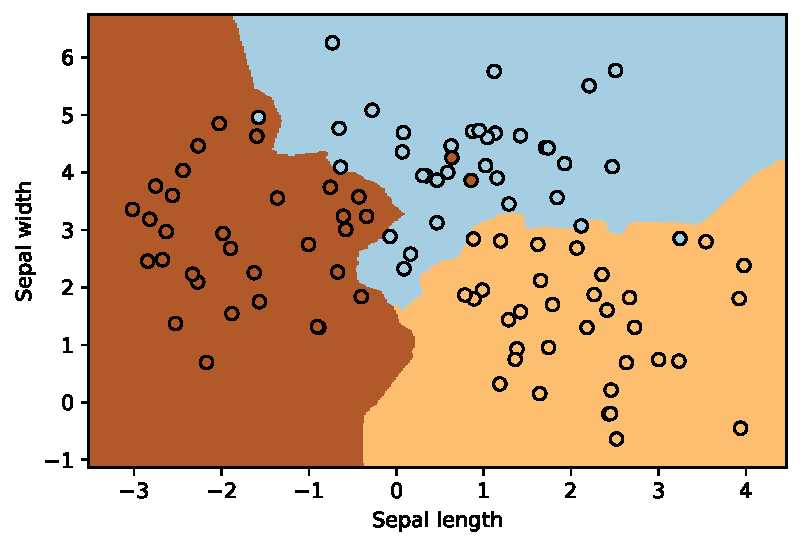
\includegraphics[height=0.7\textwidth]{../assets/knn/figures/iris_knn_5.pdf}\captionof{figure}{K = 5}\end{column}\end{columns}}
%\only<3>{\begin{columns}[T]
%  \begin{column}{0.5\textwidth}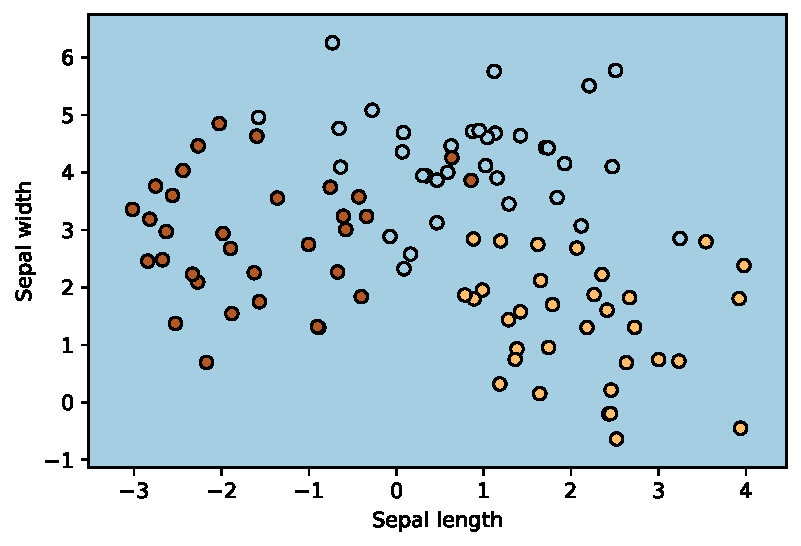
\includegraphics[height=0.7\textwidth]{../assets/knn/figures/iris_knn_100.pdf}\captionof{figure}{K = 100}\end{column}
%  \begin{column}{0.5\textwidth}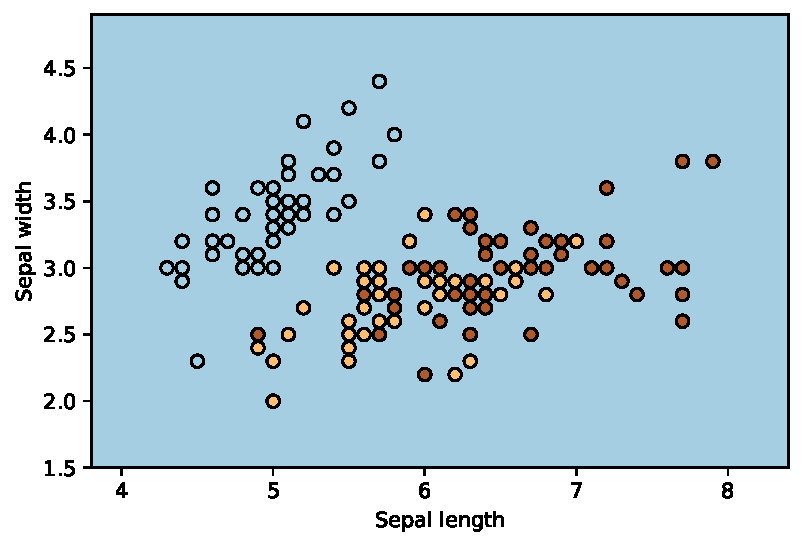
\includegraphics[height=0.7\textwidth]{../assets/knn/figures/iris_knn_150.pdf}\captionof{figure}{K = 150}\end{column}\end{columns}}
%\end{frame}
\begin{comment}


\begin{frame}{Important Considerations: Aggregation Functions}
\only<1-2>{There are different ways to go about aggregating the data from the K nearest neighbors.}

\only<2>{\vspace{0.5cm} One method to do so would be to calculate the mean and choose the class that has the highest probability.}
\only<3>{\vspace{0.5cm}\begin{figure}
      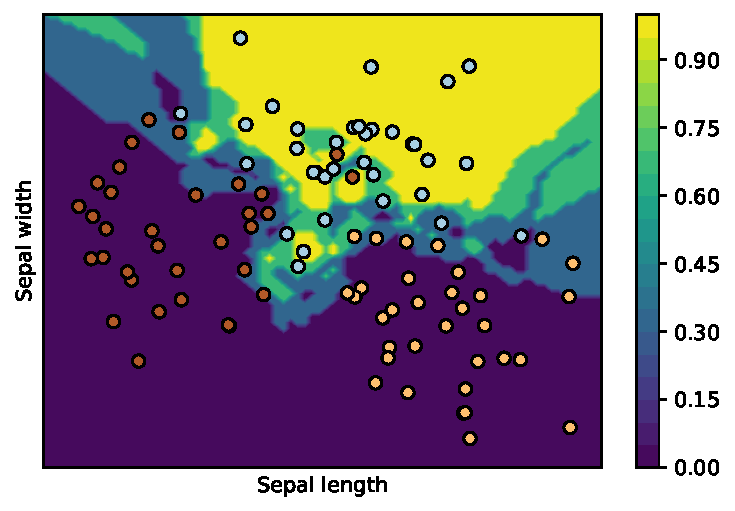
\includegraphics[width=0.8\textwidth]{../assets/knn/figures/iris_prob_3_0.pdf}
      \caption{Probability Distribution for a point to belong to Class 0}
    \end{figure}
}

\only<4>{\vspace{0.5cm}\begin{columns}[T]
  \begin{column}{0.33\textwidth}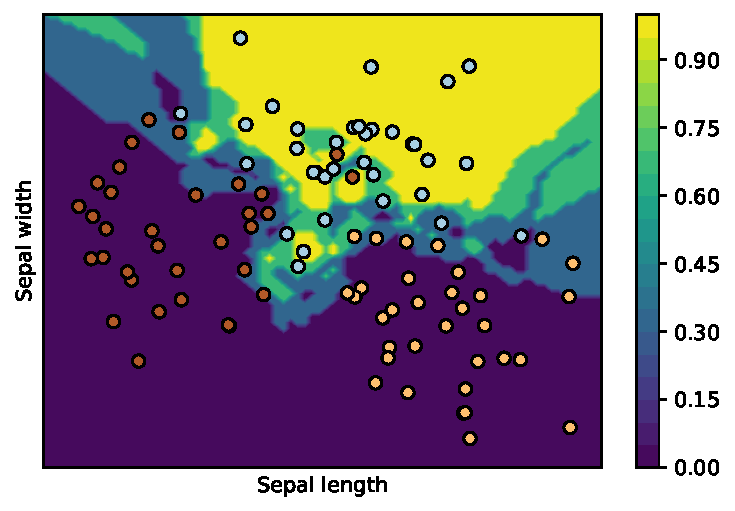
\includegraphics[height=0.7\textwidth]{../assets/knn/figures/iris_prob_3_0.pdf}\captionof{figure}{K = 3 Class 1}\end{column}
  \begin{column}{0.33\textwidth}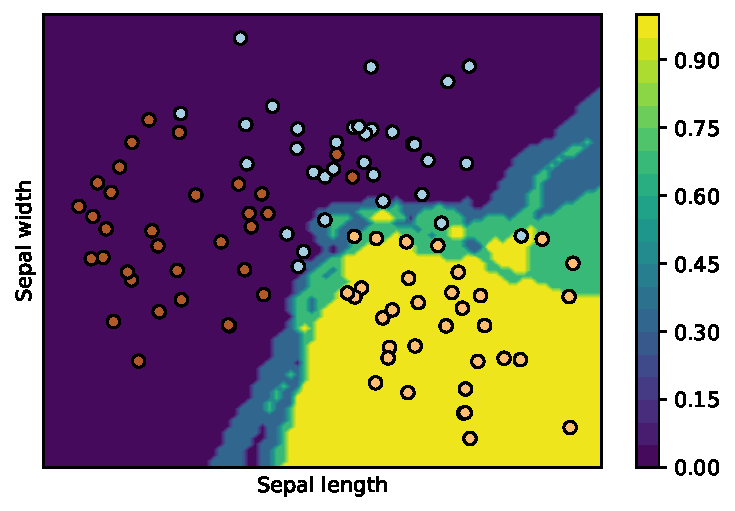
\includegraphics[height=0.7\textwidth]{../assets/knn/figures/iris_prob_3_1.pdf}\captionof{figure}{K = 3 Class 2}\end{column}\begin{column}{0.33\textwidth}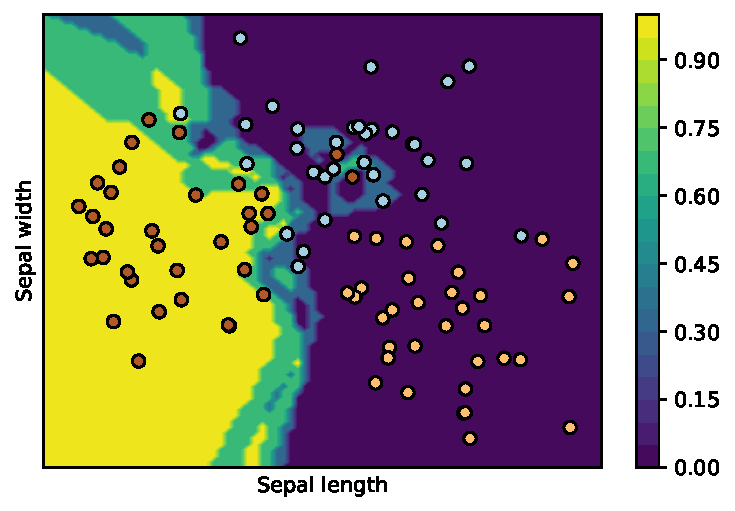
\includegraphics[height=0.7\textwidth]{../assets/knn/figures/iris_prob_3_2.pdf}\captionof{figure}{K = 3 Class 3}\end{column}\end{columns}
  \vspace{1cm}
  \begin{columns}[T]
  \begin{column}{0.33\textwidth}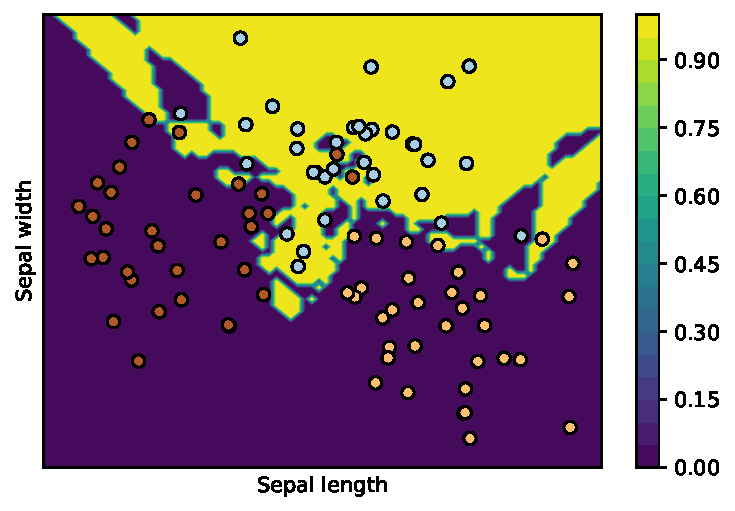
\includegraphics[height=0.7\textwidth]{../assets/knn/figures/iris_prob_1_0.pdf}\captionof{figure}{K = 1 Class 1}\end{column}
  \begin{column}{0.33\textwidth}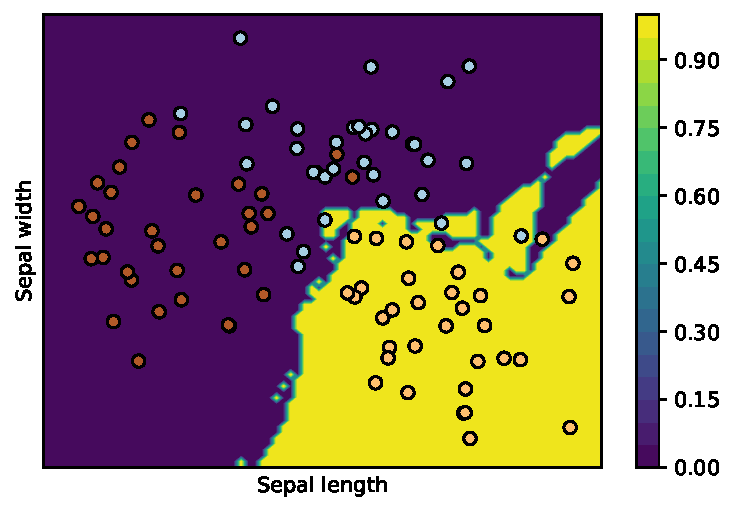
\includegraphics[height=0.7\textwidth]{../assets/knn/figures/iris_prob_1_1.pdf}\captionof{figure}{K = 1 Class 2}\end{column}\begin{column}{0.33\textwidth}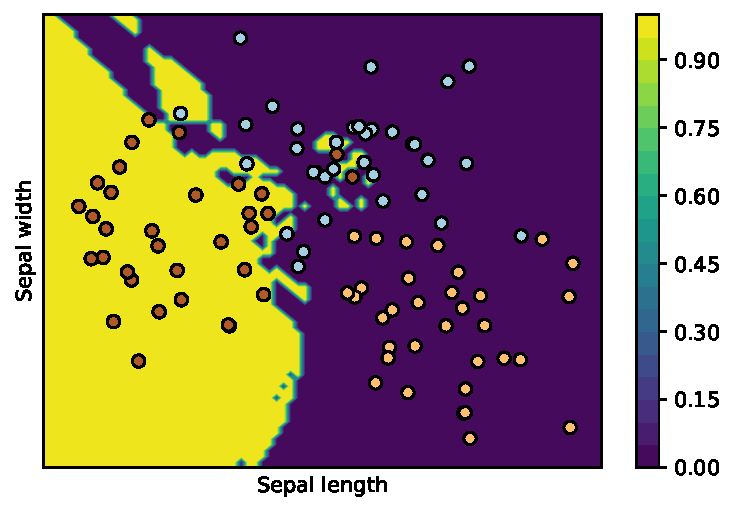
\includegraphics[height=0.7\textwidth]{../assets/knn/figures/iris_prob_1_2.pdf}\captionof{figure}{K = 1 Class 3}\end{column}\end{columns}}
  
\only<5>{
There are different ways to go about aggregating the data from the K nearest neighbors.

\vspace{0.5cm} One method to do so would be to calculate the mean and choose the class that has the highest probability.

\vspace{0.5cm} Other methods include:
\begin{itemize}
\item Median
\item Mode
\end{itemize}
}
\end{frame}
\end{comment}

\begin{frame}{Aggregating data}
	There are different ways to go about aggregating the data from the K nearest neighbors.
	
	
	\begin{itemize}
		\item Median
		\item Mean
		\item Mode
	\end{itemize}
\end{frame}
\begin{frame}{KNN Algorithm}
\begin{itemize}
\item<1-> Keep the entire dataset: ${(x,y)}$
\item<2-> For a query vector $q$:
\begin{enumerate}
\item<3-> Find the k-closest data point(s) $x^*$
\item<4-> Predict $y^*$
\end{enumerate}
\end{itemize}
\end{frame}

\begin{frame}{Curse of Dimensionality}
With an increase in the number of dimensions:
\begin{enumerate}
\item<2-> the distance between points starts to increase
\item[]<2> {\centering 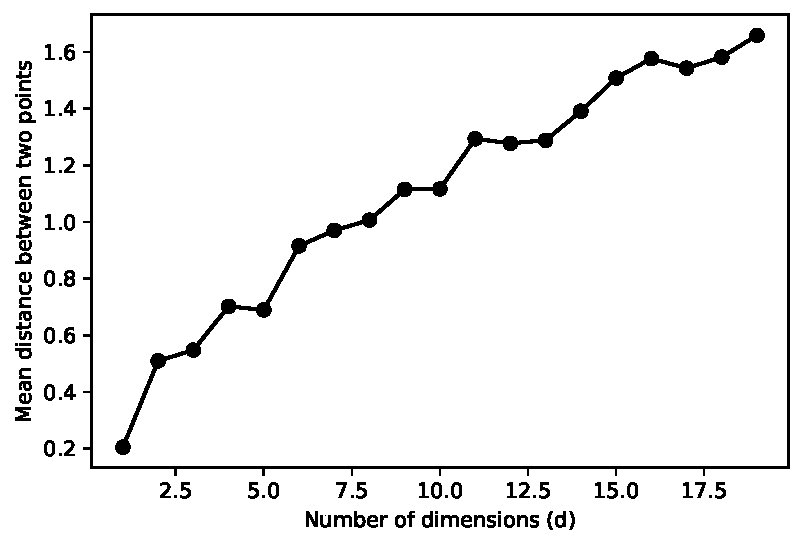
\includegraphics[height=0.6\textheight]{../assets/knn/figures/curse_dist.pdf}}
\captionof{figure}{For a unifromly random dataset}
\end{enumerate}
\end{frame}

\begin{frame}{Curse of Dimensionality}
With an increase in the number of dimensions:
\begin{enumerate}
\item the distance between points starts to increase
\item the variation in distances between points starts to decrease
\item[] {\centering 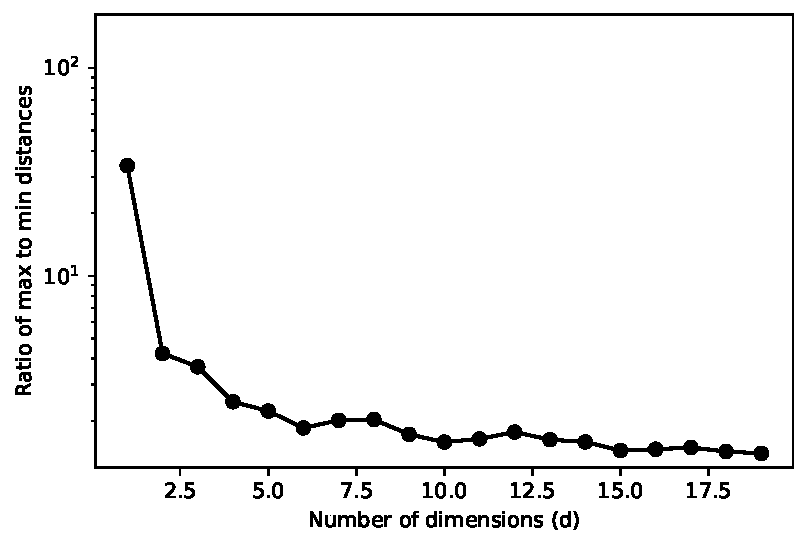
\includegraphics[height=0.6\textheight]{../assets/knn/figures/curse_spread.pdf}}
\captionof{figure}{For a unifromly random dataset}
\end{enumerate}
\end{frame}

\begin{frame}{Curse of Dimensionality}
With an increase in the number of dimensions:
\begin{enumerate}
\item the distance between points starts to increase
\item the variation in distances between points starts to decrease
\end{enumerate}
Due to this, distance metrics lose their efficacy as a similarity metric.
\end{frame}

\begin{frame}{Approximate Nearest Neighbors}
\only<1>{\vspace{0.5cm}
Doing an exhaustive search over all the points is time consuming, especially if you have a large number of data points.
\begin{figure}
      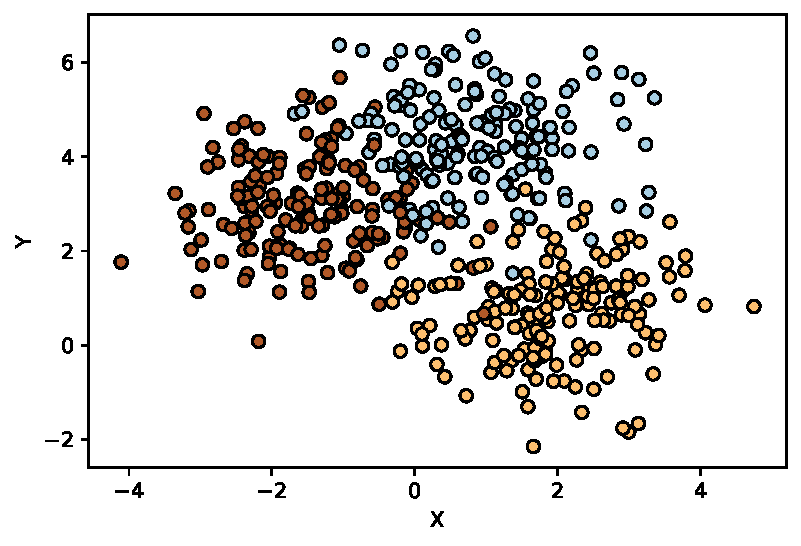
\includegraphics[width=0.6\textwidth]{../assets/knn/figures/big.pdf}
      \caption{Example of a big dataset}
    \end{figure}}
\only<2->{
Doing an exhaustive search over all the points is time consuming, especially if you have a large number of data points.

If you are willing to sacrifice accuracy there are algorithms that can give you improvements that go into orders of magnitude.
}

\only<3->{
Such techniques include:
\begin{itemize}
\item<4-> Locality sensitive hashing
\item<5-> Vector approximation files
\item<6-> Greedy search in proximity neighborhood graphs
\end{itemize}
}
\end{frame}

\begin{frame}{Locality sensitive hashing}
\vspace{0.5cm}
\only<1-2>{Normal hash functions $H(x)$ try to keep the collision of points across bins uniform.}

\only<2->{A locality sensitive hash (LSH) function $L(x)$ would be designed such that similar values are mapped to similar bins. }

\only<3->{For such cases, all elements in a bin would be given the same label, which again can be decided on the basis of different aggregation methods}

\only<1->{
\begin{figure}
      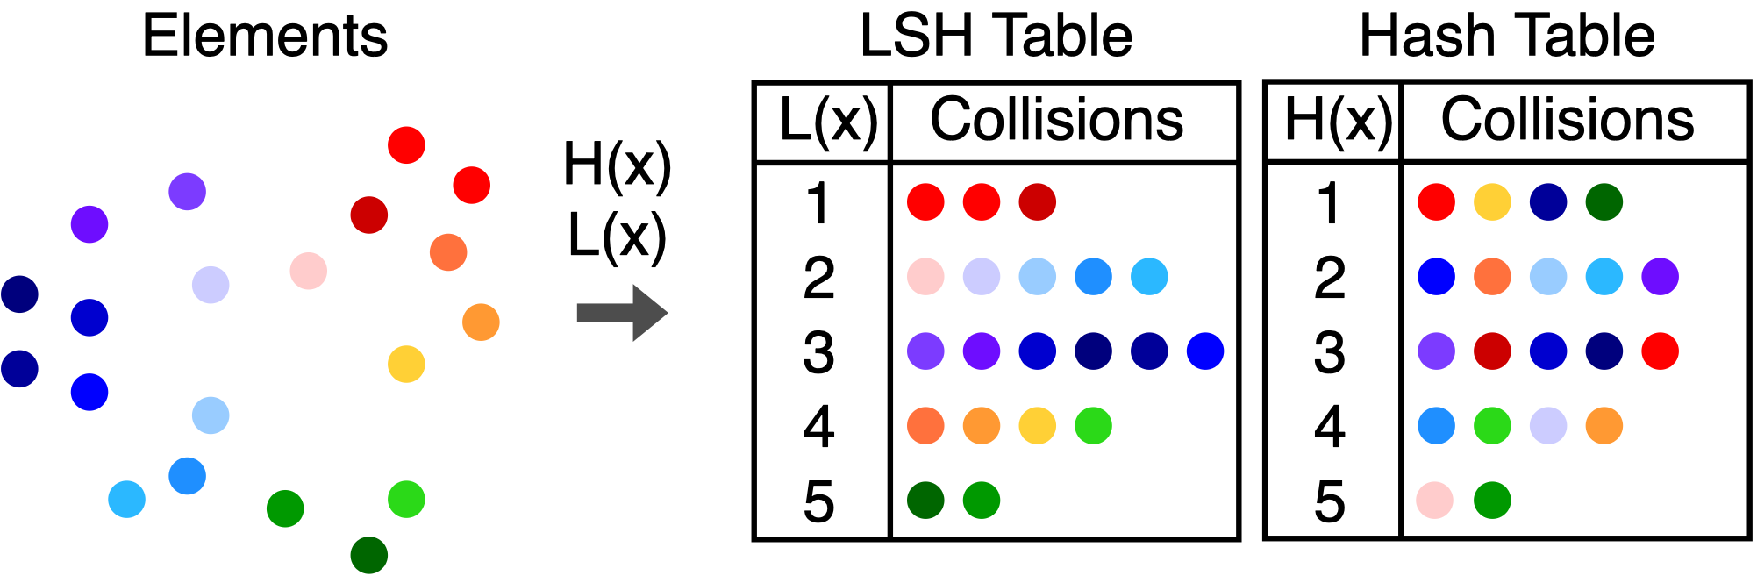
\includegraphics[width=0.8\textwidth]{../assets/knn/figures/lsh.pdf}
      \caption{Example of a big dataset}
    \end{figure}}
\end{frame}

{
	\setbeamercolor{background canvas}{bg=}
	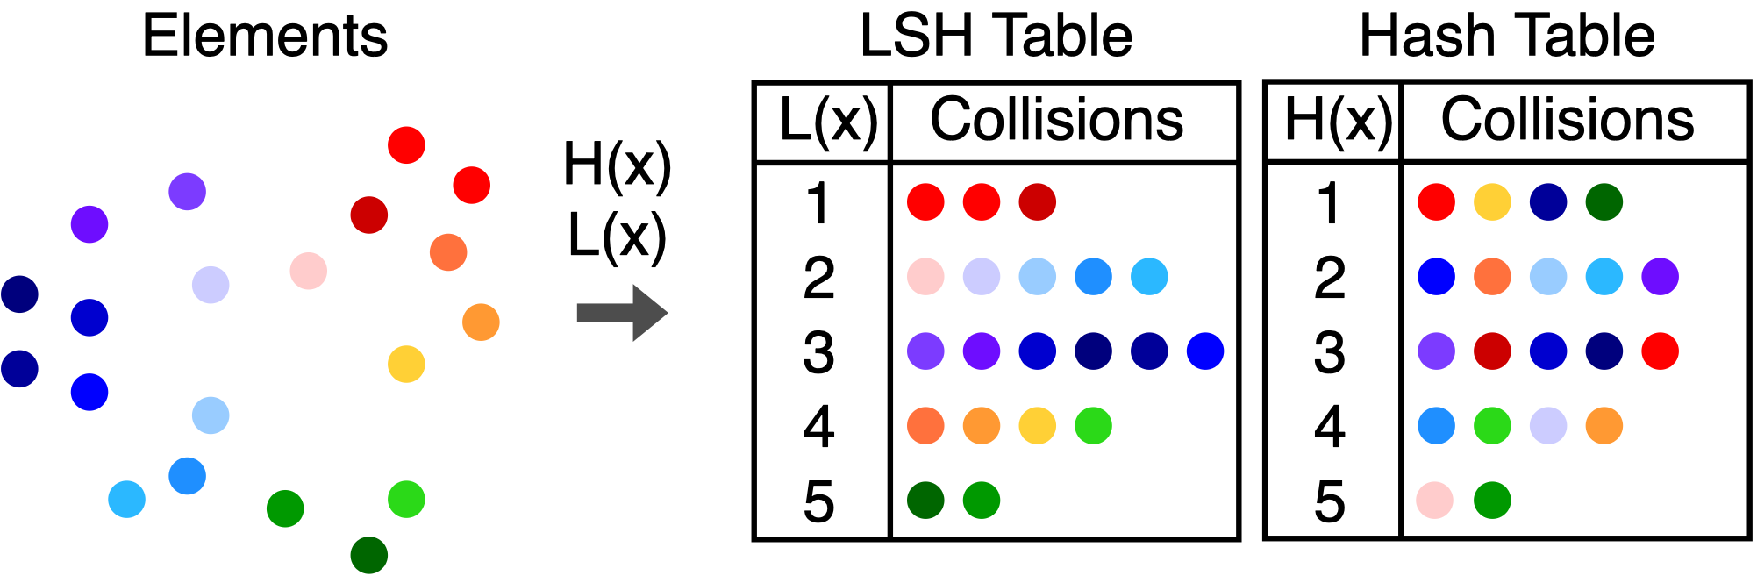
\includepdf[page=-]{../assets/knn/figures/LSH-example.pdf}
}
\end{document}
